\documentclass[12pt]{article}
\usepackage{geometry}                % See geometry.pdf to learn the layout options. There are lots.
\geometry{letterpaper}                   % ... or a4paper or a5paper or ... 
%\geometry{landscape}                % Activate for for rotated page geometry
\usepackage[parfill]{parskip}    % Activate to begin paragraphs with an empty line rather than an indent
\usepackage{daves,fancyhdr,natbib,graphicx,dcolumn,amsmath,lastpage,url}
\usepackage{amsmath,amssymb,epstopdf,longtable}
\DeclareGraphicsRule{.tif}{png}{.png}{`convert #1 `dirname #1`/`basename #1 .tif`.png}
\pagestyle{fancy}
\lhead{CE 5362 -- Surface Water Modeling}
\rhead{SPRING 2009}
\lfoot{REVISION NO. 1}
\cfoot{}
\rfoot{Page \thepage\ of \pageref{LastPage}}
\renewcommand\headrulewidth{0pt}



\begin{document}
\begin{center}
{\textbf{{ CE 5362 Surface Water Modeling} \\ {Essay 4.1}}}
\end{center}

\tableofcontents

\section{Cell Balance Model --- Volume Balance in a Tank}
This essay examines how to simulate the time to drain a tank.  This particular example is a variation of a  common problem in hydraulic engineering courses to motivate the concept of control volumes and the conservation of mass.  The equations of motion are usually given (as they are here) based on an assumption of negligible energy loss as the tank drains\footnote{Bernoulli's equation.}.

The purpose is to gain some practice with numerical modeling techniques before trying the Lax-Scheme for the 1D dynamic flow equations in an open channel.

\section{Problem Description}
Consider the tank depicted in Figure \ref{fig:time2drain.pdf}.  The water depth in the tank at any instant is $z(t)$.  The tank cross-section area is $A_{tank}$ and the outlet cross section area is $A_{out}$.   The product of $A_{tank}$ and $z(t)$ is the volume in storage in the tank at some instant, and the outflow from the tank is $Q(t)$.
\begin{figure}[h!] %  figure placement: here, top, bottom, or page
   \centering
   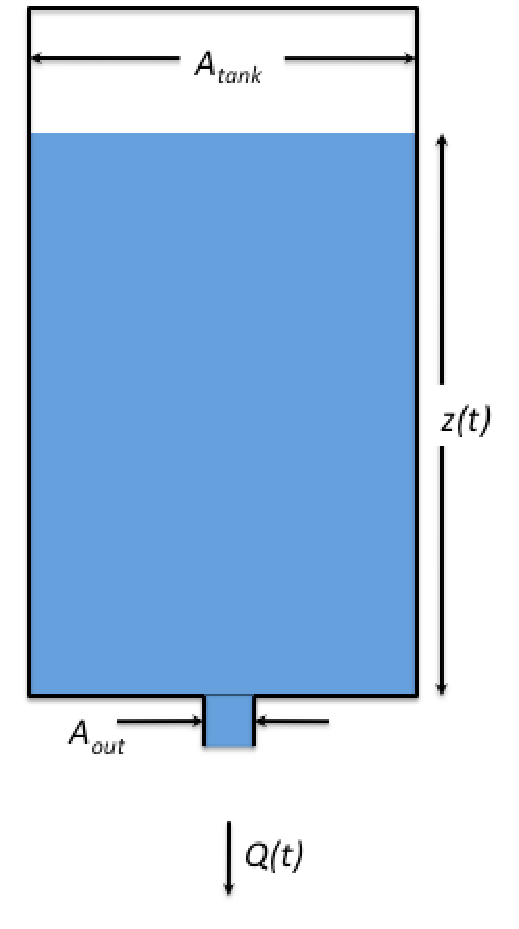
\includegraphics[width=3in]{time2drain.pdf} 
   \caption{Storage tank with drain on bottom.}
   \label{fig:time2drain.pdf}
\end{figure}


As a first model consider the computation of 
\begin{enumerate}
\item Time to drain the tank from a known initial depth.
\item Storage in the tank at some given time.
\item Depth in tank at some given time.
\item Discharge rate at some instant in time.
\item How long to drain the tank to $\frac{1}{2}$ or $\frac{1}{4}$ full.
\end{enumerate}

All these questions are reasonable kinds of questions that could arise in some engineering design situation or (more likely) in an operations scenario. In this example the tank has constant cross section, but it is not a far stretch to imagine that the tank could represent a reservoir of variable geometry.  A practical reason to ask such questions arises in storm-water detention pond design (as well as reactor design in wastewater when dynamic flows are considered) --- the time to drain impacts the remaining capacity in a detention pond, the remaining capacity is what provides some measure of control for back-to-back storms.  If the tank drains too slowly, there will not be enough reserve for a back-to-back storm, whereas if the tank drains too fast it is hydraulically irrelevant.

While this problem seems detached from an open channel flow course, it [the problem] is not.  Each node in the open channel equations where flow depth is computed is essentially such a tank.  The tank area is not constant (instead the area is related to depth and reach distance), but like this tank the inflows and outflows are, in-part, governed by the depth already in the tank.


\section{Computational Approach}
This example will be handled first analytically (because it is simple to do so), then by a simple finite-difference scheme.  For pedagogical reasons, the solutions will be computed using Excel, \textbf{R}, and \texttt{FORTRAN}.  As an ``advanced'' trick, this example will also show how to use \textbf{R} as a pre- and post-processor for a \texttt{FORTRAN} program to take advantage of the graphics package in \textbf{R}, and the huge library of existing \texttt{FORTRAN} solutions.

\subsection{Problem Analysis --- Development of the Analytical Solution}
To write an equation or set of equations for this problem, the relationship of tank depth, areas, and discharges must be specified.

If we write Bernoulli's equation along a streamline in the tank from the free surface to the outlet we would arrive at something like
\begin{equation}
\frac{p_{fs}}{\gamma}+\frac{V_{fs}^2}{2g}+z_{fs} = \frac{p_{out}}{\gamma}+\frac{V_{out}^2}{2g}+z_{out}
\label{eqn:tank_bernoulli}
\end{equation}

If we invoke the following reasonable assumptions:
\begin{enumerate}
\item $p_{fs}~=~0$ Free surface at zero gage pressure.
\item $p_{out}~=~0$ Pressure in jet is $\approx~0$.
\item $V_{fs} << V_{out}$ Free surface velocity is small relative to the outlet velocity.
\item $z_{out}~=~0$ the outlet is the datum.
\end{enumerate}

The resulting relationship between depth, and discharge is
\begin{equation}
Q(t)=A_{out} \times \sqrt{2gz(t)}
\label{eqn:tank_discharge}
\end{equation}

Now we have an equation of motion.  A mass balance in the tank requires that the storage decrease as the tank drains. Thus relating the change in tank depth and discharge produces the ordinary differential equation (ODE) that governs (at least in our model world) the tank.

\begin{equation}
A_{out} \times \sqrt{2gz(t)}=-A_{tank} \times \frac{d z}{d t}
\label{eqn:tank_ode}
\end{equation}

If one collects the constants $\frac{-A_{out}}{A_{tank}}\sqrt{2g} = \alpha$ the ODE is a little simpler to examine\footnote{The constants can be collected in this case because the geometry stays constant in the tank --- changing geometries would have areas as functions of depth and could not be collected in this fashion.}

\begin{equation}
\alpha  [z(t)]^{\frac{1}{2}}=  \frac{d z}{d t}
\label{eqn:tank_characteristic_ode}
\end{equation}

Equation \ref{eqn:tank_characteristic_ode} can be separated and integrated

\begin{equation}
\int_0^T{\alpha~dt }= \int_{z(0)}^0{ \frac{d z}{ [z(t)]^{\frac{1}{2}}} }
\label{eqn:tank_characteristic_integrated}
\end{equation}

The solution is

\begin{equation}
z(t)=(z(0)^{\frac{1}{2}}-\frac{\alpha}{2}t)^2
\label{eqn:tank_characteristic_solution}
\end{equation}

\subsection{Problem Analysis --- Development of the Finite-Difference Approximation}
The finite difference approximation follows the same principles up to Equation \ref{eqn:tank_characteristic_ode} then approximates the derivative term by its difference quotient for small time steps\footnote{Recall the fundamental theorem of calculus where the difference quotient is taken to the limit and this limit is called the derivative --- here we don't go to the limit, instead using small but finite steps.}

\begin{equation}
\alpha  [z(t)]^{\frac{1}{2}}\approx~  \frac{\Delta z}{\Delta t}
\label{eqn:tank_characteristic_fda}
\end{equation}

Notice some features of \ref{eqn:tank_characteristic_fda}.  First the equal sign is changed to ``approximately'' equal; second the derivative is changed to a related rate.  The remainder of the ``equation'' is unchanged.  The trick here is to understand how to interpret the equation. 
\begin{quote}
The approximation states that the rate of change of depth with time is approximately equal to the product of the geometric and gravitational constant and the square root of the current depth. 
\end{quote}

Using this approximation, and knowing the depth in the tank to start produces an algorithm to explore the tank behavior.  First expand the difference equation.
\begin{equation}
\alpha  [z(t)]^{\frac{1}{2}}= \frac{z(t+\Delta t) - z(t) }{\Delta t}
\label{eqn:tank_expanded_fda}
\end{equation}

Then rearrange to isolate values at time $t+\Delta t$,

\begin{equation}
{z(t+\Delta t) } = z(t) + \Delta t \alpha  [z(t)]^{\frac{1}{2}}
\label{eqn:tank_update}
\end{equation}

All the terms on the right hand side are known and the equation\footnote{Now known as an update equation} tells the modeler how to approximate depth at a future time.  Because the analysis assumed the difference quotient is close to the derivative, the time steps need to be kept pretty small (in fact in many problems the time step is constrained by the physics for stability and by the computation regime for precision).

The particular update here is an implementation of Euler's method\footnote{One of many methods to approximate solutions to ordinary differential equations}.  There are other methods --- the reader should observe that the time difference scheme could be backwards so that the discharge could be at an unknown time, or a weighted average of the two times, or a variety of other ways to approximate the derivative.

\section{Application of Analytical Solution}
This section presents the analytical solution coded in Excel, \textbf{R}, and \texttt{FORTRAN}.  
\subsection{Excel Implementation}
The Excel implementation is straightforward.  Put the formula in equation \ref{eqn:tank_characteristic_solution} into each cell of the spreadsheet and supply correct references to the constants and the time.  The solution is a quadratic equation and has a minimum value of zero at some time (the time to drain) and beyond this time the computed depth starts to increase again --- once the minimum value is passed the solution has no physical significance.

\begin{figure}[h!] %  figure placement: here, top, bottom, or page
   \centering
   \includegraphics[width=6in]{excelAnalForm.pdf} 
   \caption{Analytical result in Excel (as formulas).}
   \label{fig:excelAnalForm}
\end{figure}

\begin{figure}[h!] %  figure placement: here, top, bottom, or page
   \centering
   \includegraphics[width=6in]{excelAnalNum.pdf} 
   \caption{Analytical result in Excel (as values --- the usual presentation)}
   \label{fig:excelAnalNum}
\end{figure}

The actual time to drain can be found by trial-and-error, or simply by minimizing equation \ref{eqn:tank_characteristic_solution} with respect to time.

\subsection{\textbf{R} Implementation}
Analytical solutions are usually straightforward to represent in environments like \textbf{R}.  In this example, a single line of code builds the relationship and a couple more lines for a plot.

\begin{verbatim}
> depth<-function(alpha,time,initialDepth){(sqrt(initialDepth)-0.5*alpha*time)^2}
> tt<-seq(1,1000)
> plot(tt,depth(alpha,tt,5),xlab="Time (minutes)",ylab="Depth (meters)")
\end{verbatim}

The actual ``plot'' is left as an exercise. 

\subsection{\texttt{FORTRAN} Implementation}
A \texttt{FORTRAN} implementation is also fairly straightforward --- using Excel as the structural example a simple code to simulate the time to drain could be:

\begin{verbatim}
      program time2drain_analytical
c========
c Author: T.G. Cleveland
c Date:   2008_0104
c Purpose: Pedagogical tool for CE 5362
c
c====Time to drain by analytical expression====
c     produces two columns: time and depth
c    input:  depth1, areaT, areaO, tprt
c      depth1 = initial depth at time zero
c      areaT = tank area
c      areaO = outlet area
c      tprt = print frequency ( a time step )
c====Spacing guide
c23456789012345678901234567890
c        1         2         3
c====Declare Variables====
      real*8 depth1,areaT,areaO,tprt
      real*8 alpha
      real*8 time(1000),depth(1000)
c====Read from STDIO (redirection)====
      read(*,*)depth1,areaT,areaO,tprt
c====Compute constant====
      alpha=sqrt(2.0D0*9.8D0)*areaO/areaT
c====Initial Conditions====
      time(1)=0.0D0
      depth(1)=depth1
c====Compute time to drain====
      tdrain=2.0D0*sqrt(depth1)/alpha
c====Now make the time series, above is stopping value====
      do 1001 irow=2,1000
	   time(irow)=time(irow-1)+tprt
c==== Exit loop test, crude programming style====
	   if(time(irow) .ge. tdrain) goto 1002
	   depth(irow)=(sqrt(depth1) - 0.5D0*alpha*time(irow))**2
 1001 continue
c===If normal exit more time remains====
c===Would normally report in this block and do someting====
 1002 continue
c===Prepare and write the output to STDIO (redirection)====
      write(*,*)'time','  ','depth'
      do 1003 jrow=1,irow-1
       write(*,*)time(jrow),depth(jrow)
 1003 continue
      stop
      end
\end{verbatim}

Once this program is coded the analyst would them prepare an input file (or enter directly from the command line) and redirect to an output file.  The next two figures illustrate each approach.

\begin{figure}[h!] %  figure placement: here, top, bottom, or page
   \centering
   \includegraphics[width=6in]{fortANL_T1.pdf} 
   \caption{Analytical result in \texttt{FORTRAN}.}
   \label{fig:fortANL_T1.pdf}
\end{figure}

First, direct interaction is displayed in Figure \ref{fig:fortANL_T1.pdf}.  Notice the compilation step, then running the program.  The command line is blank until we enter the four input values and the machine will wait until the end of time unless we send it the data (or an interrupt command).  The output is sent directly to the screen.

Second, through files and redirection (the better way!) we can capture the output and send different data streams (if we wish).  This redirection approach (an extremely important modeling concept!) is illustrated in Figure \ref{fig:fortranANYL_RED.pdf}.  The source code is the same as before.  The input file named \texttt{tank.txt} is an ASCII text file with the five data elements (the numbers) and some extra text\footnote{This extra text is not read by the program and is a convenience for the modeler to remember what each data element means --- think of these as tags or labels associated with the data.  The program does not read these because of the way list directed reads work in ANSI FORTRAN.  In other situations the extra text will cause the program to abort.}.

\begin{figure}[h!] %  figure placement: here, top, bottom, or page
   \centering
   \includegraphics[width=6.in]{fortranANYL_RED.pdf} 
   \caption{Analytical result in \texttt{FORTRAN} using files and redirection}
   \label{fig:fortranANYL_RED.pdf}
\end{figure}

The program is NOT recompiled --- there is no need.  The command line that runs the program has an interesting structure worth examination:

$\dots$ \texttt{./time2drainANL.exe < tank.txt > tank.out.txt}  is the actual command to run the program.  

The symbol \texttt{<} tells the operating system to redirect the contents of the file that follows this symbol into the program.  

The symbol \texttt{>} tells the operating system to redirect the program output that would go to the screen into the file whose name follows the symbol.  

The input redirection file must exist, the system will create the output file if it does not exist.  If the input file does not have the data in a structure the program understands the program will abort and usually send to the standard error (a different device than standard input/output) device an error message --- relatively undecipherable until the modeler has a lot of experience.  Most of the time programs fail is because the input files get garbled.

In addition to garbled input files (missing an element, etc.) files created in MS Windows environments have a different line-feed structure than files created in Linux/UNIX or Macintosh.  A useful sequence of events if a program ran with one file and failed with another file with different numbers but apparently the same structure is to check if the files came from a foreign (to the host) operating system.

There is a useful Linux/UNIX utility (which will run in CYGWIN\footnote{Cygwin is a Linux-like environment for Windows. It consists of two parts: A DLL (cygwin1.dll) which acts as a Linux API emulation layer providing substantial Linux API functionality, and a collection of tools which provide Linux look and feel. \textbf{http://www.cygwin.com/}}) that converts the files.  The utility is called \texttt{dos2unix} and \texttt{unix2dos}.  The utility can be found on the internet.

A final comment about redirection, Linux/UNIX, Windows, Mac OS X, OS 2, VAX-VMA, Solaris, WInCE, etc. all use and support redirection; in fact redirection is the essence of object oriented programs.  The syntax at the command line is similar in all these environments.  Redirection allows code to be reused and only the data stream are changed.

\section{Application of the Finite-Difference Approximation}
This section presents the same set of ``solutions'' using the finite-difference model.  In these cases the underlying algorithm is that expressed by Equation \ref{eqn:tank_update}.

\subsection{Excel Implementation}
The Excel implementation is straightforward.  As before put the update formula in into each cell of the spreadsheet and supply correct references to the constants and the time.  In this model we code in a test to prevent taking the square root of negative numbers (which generates \texttt{NAN} errors).

\begin{figure}[h!] %  figure placement: here, top, bottom, or page
   \centering
   \includegraphics[width=5in]{excelFDMF.pdf} 
   \caption{Finite-Difference result in Excel (as formulas).}
   \label{fig:excelFDMF}
\end{figure}

Figure \ref{fig:excelFDMF} is an example spreadsheet with the cells containing the formulas used to compute the depth-time relationship from the finite-difference update equation.  Notice the logical test imbedded in the formulas.

\begin{figure}[h!] %  figure placement: here, top, bottom, or page
   \centering
   \includegraphics[width=5in]{excelFDMNum.pdf} 
   \caption{Finite-Difference result in Excel (as values --- the usual presentation)}
   \label{fig:excelFDMNum}
\end{figure}

Figure \ref{fig:excelFDMNum} is the same spreadsheet with values displayed.  There is little visible difference in these figures between the analytical and numerical spreadsheets, but the underlying concepts are quite different.  

\subsection{\textbf{R} Implementation}
To model the tank using \textbf{R} the modeler needs to write the necessary equation structure in the proper order.  Below is a crude implementation --- note how the update quotient is actually built with a test for near zero values to prevent attempted square root of a negative number.   Also note how there is some flexibility to change the time step.

\begin{verbatim}
> # Time to Drain Model
> AreaTank<-987
> AreaPipe<-1
> alpha<-sqrt(2*9.8)*AreaPipe/AreaTank
> z<-numeric(0)  # define the depth array
> z[1]<-5.0 # initial depth
> dt<-5.0 # time step size
> # program the update difference quotient
> dzdt<-function(alpha,depth){if(depth >= 0.001)alpha*sqrt(depth) else 0}
> # update many times
> for (i in 1:500){z[i+1]=z[i]-dt*dzdt(alpha,z[i])}
> length(z) # get length for plotting
[1] 501
> time<-seq(0,500)*dt
> plot(time,z,xlab="Time (minutes)",ylab="Depth (meters)")
\end{verbatim}

The result of the plot call is displayed in Figure \ref{fig:Time2DrainR.pdf}

\begin{figure}[htbp] %  figure placement: here, top, bottom, or page
   \centering
   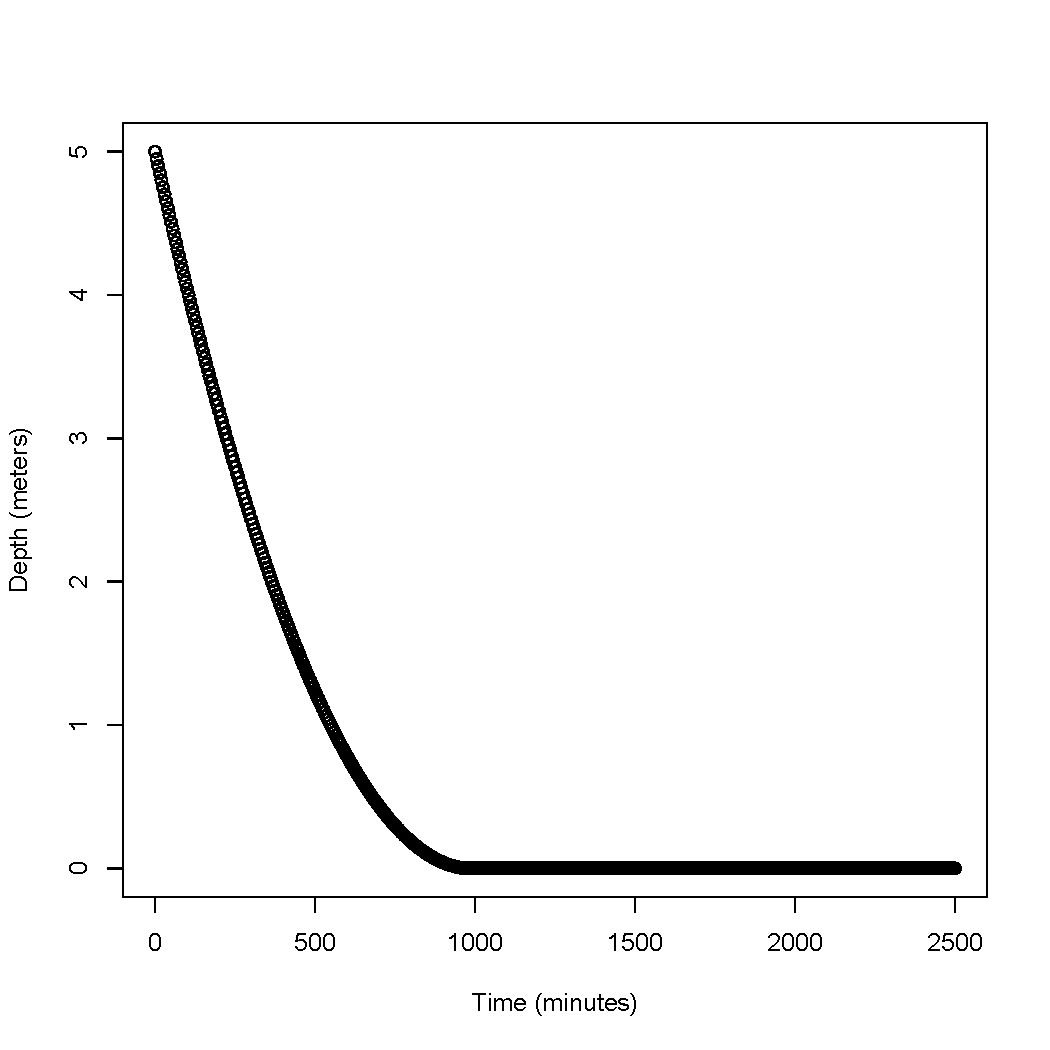
\includegraphics[width=5in]{Time2DrainR.pdf} 
   \caption{Plot of relationship of elapsed time and depth of water in tank.}
   \label{fig:Time2DrainR.pdf}
\end{figure}

The plot displays a lot of zero values, the student should explore tricks to plot only the interesting portion of the behavior.  The student should also explore how to plot both the analytical and numerical solution on the same graph.

\subsection{\texttt{FORTRAN} Implementation}
To model the tank using \texttt{FORTRAN} the modeler needs to write \texttt{FORTRAN} source code, compile and link the code, then run the code.  Input and output need to be handled by redirection or file read/writes.  

First, here is working source code:
\begin{verbatim}
      program time2drain
c====time to drain a tank model
c
c Author: T.G. Cleveland
c Date:   2009_0105
c Purpose: Pedagogical tool for CE 5362 Surface Water Modeling
c
c====variable names:
c    depth = tank depth (an array)
c    time = elapsed time (an array)
c    tankArea = tank surface area (a constant)
c    pipeArea = pipe area (a constant)
c    deltaTime = time step length (a constant)
c
c==== Program testing
c    Works as written using Windows MS Powerstation Fortran
c    Works as written using Windows GNU FORTRAN
c    Works as written using Linux/UNIX g77 FORTRAN
c    Works as written using GNU Fortran 95 (Mac OS X) 
c=== Spacing guide  
c23456789012345678901234567890
c        1         2         3
c====declare variables====
      real*8 depth
      real*8 tankArea,pipeArea,alpha
      real*8 time
      real*8 deltaTime
c====size arrays====
      dimension depth(500),time(500)
c====file name for output====
      character*14 fileout
     character*14 fileinp
      fileinp='input.txt'
      fileout='output.txt'
c==== attach files to the program ====
      open(unit=11,file=fileinp,status='old')
      rewind(11)
      open(unit=12,file=fileout,status='unknown')
      rewind(12)
c==== tank geometry, time step, and starting values ==== 
      read(11,*)tankArea
      read(11,*)pipeArea
      read(11,*)deltaTime
      read(11,*)depth(1)
      read(11,*)time(1)	  
c====characteristic geometry/acceleration term ====
      alpha=sqrt(2.0D0*9.8D0)*pipeArea/tankArea
c====begin update formula====
c====using count controlled repetition====
      do 1001 ir=2,500
       depth(ir)=depth(ir-1)-deltaTime*alpha*sqrt(depth(ir-1))
	   time(ir)=time(ir-1)+deltaTime
c====test for loop exit; crude control structure! Not recomended!
       if( depth(ir) .le. 0.001D0 )goto 1002
 1001 continue
c====write output to file====
 1002 continue
c====R expects header row====
      write(12,*)'time',' ','depth'
c====Now for the data====
      do 1003 ij=1,ir-1
       write(12,9001)time(ij),depth(ij)
 1003 continue
      stop
 9001 format(f10.3,2x,f10.3)
      end
 \end{verbatim}
 
The program as written is pretty crude \texttt{FORTRAN} but suitable for this essay.  The reader should note that the program expects an input file names \texttt{input.txt} to be present (and populated with requisite data elements).  The program writes output to a file named \texttt{output.txt}.  These names are somewhat arbitrary and there are many other ways to handle the input/output issue.  This particular structure is to facilitate running the program from the \textbf{R} environment to take advantage of the built-in graphics.

Figure \ref{fig:fortranSC.pdf} is a screen capture of the program run in a terminal environment.  The various system commands are \texttt{head "filename"} that lists the first few lines of a file, then the actual compiling step, and then a look at the input file, and finally the first few lines of the output file.

\begin{figure}[htbp] %  figure placement: here, top, bottom, or page
   \centering
   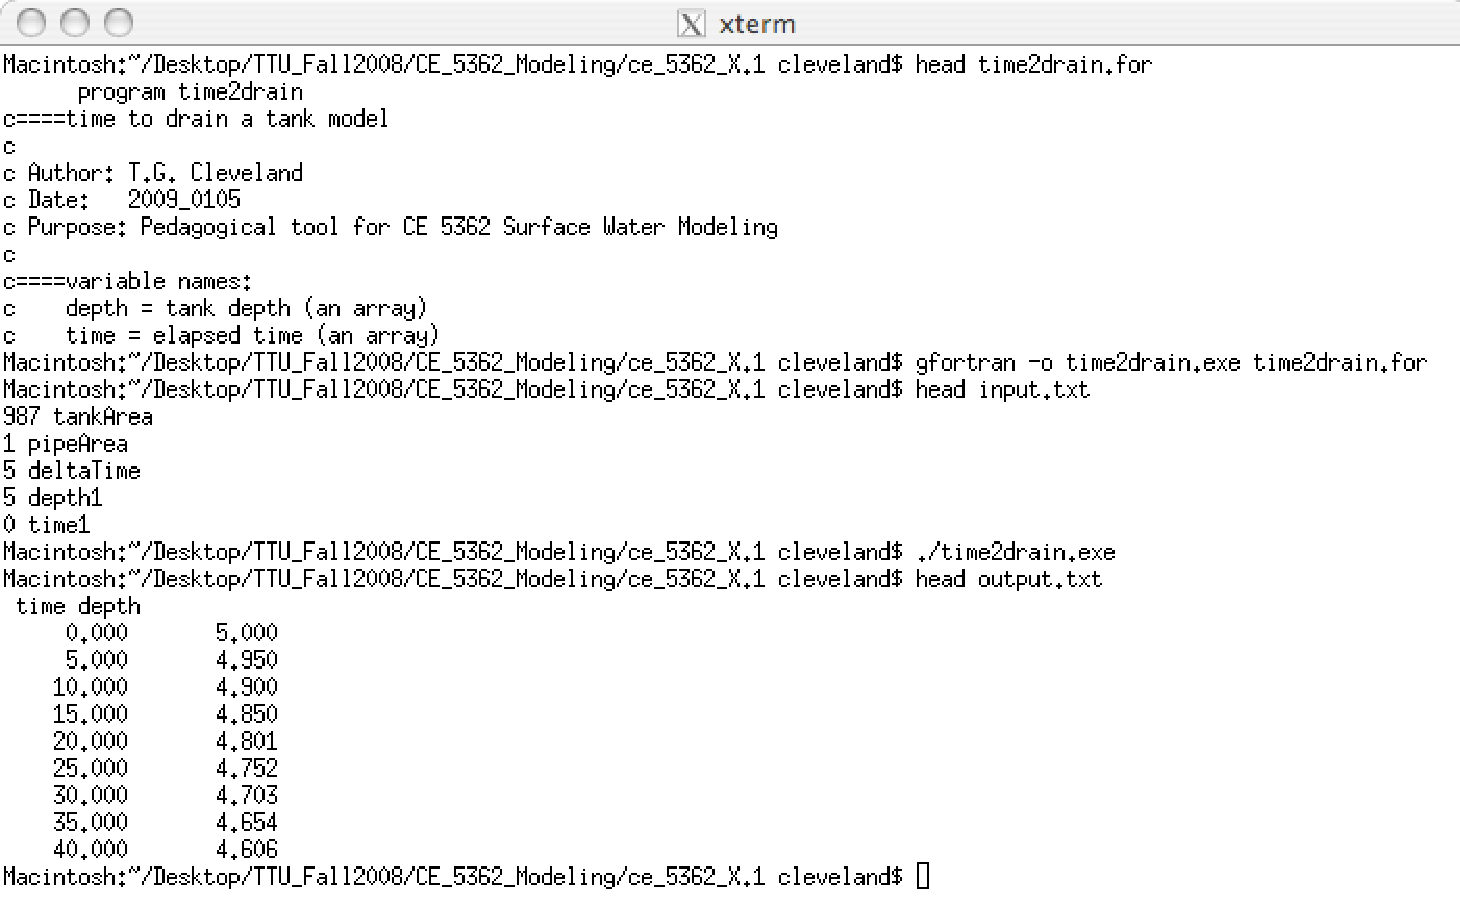
\includegraphics[width=6.5in]{fortranSC.pdf} 
   \caption{\texttt{FORTRAN} implementation for finite-difference solution.}
   \label{fig:fortranSC.pdf}
\end{figure}

In practice the next step would be to put the output file into some plotting routine (or other way to interpret).  The file could easily be read into Excel or \textbf{R} for plotting results.

\newpage

\section{Addendum: Time to drain a tank using SWMM}
SWMM in principle should be able to model a time-to-drain problem.  SWMM is certainly overkill in this respect, but worth running an example to illustrate that the tools all produce about the same answer.

The input elements into SWMM are a storage node (the tank), a short pipe (but long enough so that the program can compute non-zero head losses) and an outlet node.  A completed model is illustrated in Figure \ref{fig:swmm_tankdrain}.

\begin{figure}[htbp] %  figure placement: here, top, bottom, or page
   \centering
   \includegraphics[width=4in]{swmm_tankdrain.jpg} 
   \caption{Example SWMM model to approximate time-to-drain for a tank.  Storage element description.}
   \label{fig:swmm_tankdrain}
\end{figure}

The link information is displayed in Figure \ref{fig:swmm_tankdrainLink}.  Here a subtle trial-and-error approach was used (not displayed) to find values that produce small link head loss, yet produce correct mass balances.  The big issue (in my opinion) is the need to use a fairly large outlet pipe to simulate the holw in the bottom of the tank.  Without the analytical background, a modeler would concieviable use a smaller outlet (as indicated by the theory) and obtain a different time to drain.   Because SWMM expects real elements, the problem as stated cannot easily be studied using the tool (although as illustrated here results can be effectively mimiced).

\begin{figure}[htbp] %  figure placement: here, top, bottom, or page
   \centering
   \includegraphics[width=4in]{swmm_tankdrainLink.jpg} 
   \caption{Example SWMM model to approximate time-to-drain for a tank.  Link element description.}
   \label{fig:swmm_tankdrainLink}
\end{figure}


The output  information is displayed in Figure \ref{fig:swmm_tankplot}.  The plot has about the same shape and time-decay structure as the other plots suggesting a reasonable approximation of the process (assuming the analytical soluton is the best).

\begin{figure}[htbp] %  figure placement: here, top, bottom, or page
   \centering
   \includegraphics[width=4in]{swmm_tankplot.jpg} 
   \caption{example caption}
   \label{fig:swmm_tankplot}
\end{figure}


\newpage
\section{Addendum 2: Advanced Topic --- Accessing \texttt{FORTRAN} from \textbf{R}}
\textbf{R} like most environments can access \texttt{FORTRAN} programs either as dynamic-link-libraries or through input/output files.  Here the second approach is used, simply to take advantage of the built-in graphics in \textbf{R}. 

Here is the procedure:
\begin{enumerate}
\item Write and test the \texttt{FORTRAN} program independent of \textbf{R}.  If the program requires input, be sure the input is located in a simple file structure that \textbf{R} can generate.  In this example the program is entirely self-contained and requires no input\footnote{The generation of input from \textbf{R} into a \texttt{FORTRAN} readable file is left as an exercise.}.
\item Start \textbf{R} and set the directory to the same directory where the \textbf{compiled, operational, executable code exists!}
\item To run the \texttt{FORTRAN} program use the \textbf{R} directive \texttt{shell("program\_name.exe")}\footnote{On Unix and Mac OS X, the command is \texttt{system()}}.  There are other arguments that you can pass --- experiment.  Redirection seems to work and is worth considering for practical use.
\item Use \texttt{read.table()} to recover file contents.  Following is an example using the \texttt{FORTRAN} program for the tank drain example.
\end{enumerate}

\begin{verbatim}

># Here we set the working directory.  The FORTRAN program exists and 
> setwd("C:/Documents and Settings/Administrator/Desktop/ce_5362_X.1")
> #
> shell("time2drain.exe") # shell to OS, run the program
Stop - Program terminated.
> z<-read.table("output.txt",header=T) # Read the output file
> attach(z)
> plot(time,depth) # plot the results.
\end{verbatim}

\subsection{Building a \texttt{FORTRAN} input file}
This is same as above except the \texttt{FORTRAN} code is modified to accept an input file.  We use \textbf{R} to build the input file in a correct structure, then call the \texttt{FORTRAN} program, and plot the output.

\begin{verbatim}
> # Here's how to send data to a FORTRAN input file and run as above.
> # Be sure working directory is correct.
> getwd()
[1] "/Users/cleveland/Desktop/TTU_Fall2008/CE_5362_Modeling/ce_5362_X.1"
> # This is where the program lives!
> # The example program needs 5 data elements --- for clarity
> # I usually include a name in the input file
> y<-c("tankArea","pipeArea","deltaTime","depth1","time1")
> # y is the list of data elements the program needs. depth1 and time1 are 
> #   initial conditions, remaining terms as per the essay.
> x<-c(987,1,5,5,0) # Associated numerical values
> # Now be sure the file is non-existant
> system("rm input.txt")
> for(i in 1:5){ write(c(x[i],y[i]),file="input.txt",ncolumns=2,append=T)}
> # File is written --- use a system call to check
> system("cat input.txt")
987 tankArea
1 pipeArea
5 deltaTime
5 depth1
0 time1
> # Cool!  Correct structure --- now run the program
> system("./time2drain.exe")
> # Now read the output data and plot
> z<-read.table(file="output.txt",header=T)
> attach(z)
> # Columns should be time and depth
> plot(time,depth,xlab="Elapsed Time (seconds)",ylab="Depth (meters)")
\end{verbatim}



\section{Summary}
What this essay presented is actually quite simple.  The modeler in any case will have to conceptualize the physical system into a structure amenable to mathematical representation.  The tools are the conservation of mass, momentum, and energy.  Then relationships between components must be established --- generally time, lengths, and forces are somehow related.  These relationships, whether empirical or fundamental constitute the basis to build a model to reality.

Next the modeler has to convert these relationships into a structure that can be solved using the tools at hand: Excel, \texttt{FORTRAN}, etc.  Finally the application is built and used for the problem of interest.  While intellectually desirable to have a fairly general tool, the modeler should never be afraid to use a purpose built tool if a general tool is unavailable.  Be sure to test the tool and know its limitations.

In the essay a simple hydraulics computation was presented to motivate these modeling steps.  Solutions were constructed in three programming environments.   Each environment has its advantages and in practice the modeler should use the tool he/she knows best unless forced to use a tool by regulation or client demand.  

\section{Readings}
TBD


\section{Exercises}
\begin{enumerate}
\item Get the three example tools running on your machine.  Demonstrate that the finite-difference solution is identical using all three programming tools.  Demonstrate that the solution is close to the analytical solution.
\item Adapt the tools and build a simulator that approximates the depth of water in a cylindrical drum lying on its side as a function of time.  Figure \ref{fig:drum} is a sketch of the drum of interest. Also desired is the volume in storage in the drum as a function of time.

\begin{figure}[h!] %  figure placement: here, top, bottom, or page
   \centering
   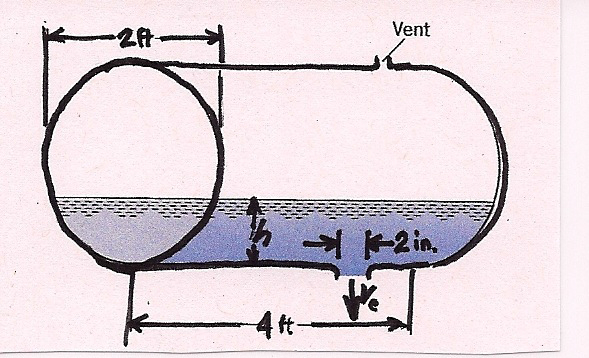
\includegraphics[width=4in]{drum.jpg} 
   \caption{Sketch of drum dimensions}
   \label{fig:drum}
\end{figure}

The drum is drained by a 2-inch diameter short pipe at the bottom of the drum.  The velocity of water in the pipe is $V_e~=~\sqrt{2~g~h}$ where $g$ is gravitational acceleration and $h$ is water depth in the tank above the outlet.  The drum is 4-feet long and 2-feet in diameter.  Simulate the time to drain from $\frac{1}{2}$ full to empty, then generalize to any starting depth (up to the tank diameter).



Produce a time versus depth and time versus storage plot for the drum using Excel and \textbf{R}.  Produce a tabulation of these values using \texttt{FORTRAN}\footnote{This exercise is to develop skill, the program needs to work and be general enough for different starting depths and different lengths and diameters.  All else can be hard coded into the program, and the \texttt{FORTRAN} to \textbf{R} interprocessing is optional.}

\item Build a simulator for a trough of arbitrary dimensions as shown in Figure \ref{fig:trough}.  

\begin{figure}[h!] %  figure placement: here, top, bottom, or page
   \centering
   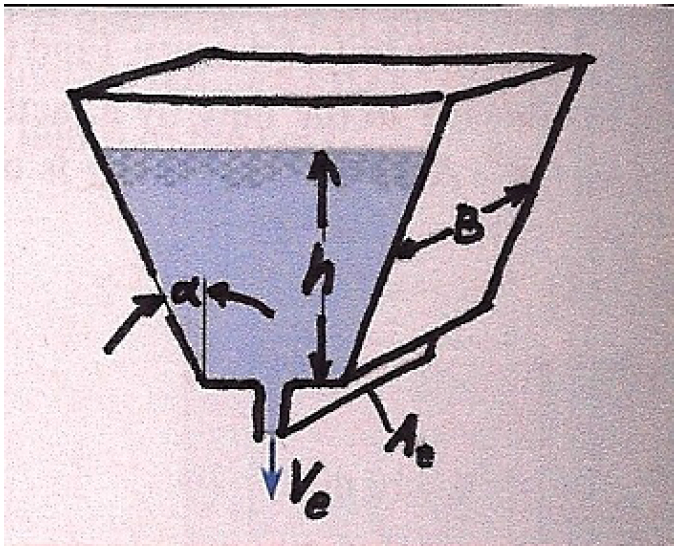
\includegraphics[width=4in]{trough.jpg} 
   \caption{Sketch of trough dimensions}
   \label{fig:trough}
\end{figure}

The angle with the vertical of the sloping sides is $\alpha$, and the distance between the parallel ends is $B$.  The width of the trough is $W_0 + 2h~tan~\alpha$, where $h$ is the distance from the trough bottom.  The velocity of water issuing from the opening in the bottom of the trough is equal to $V_e~=~\sqrt{2~g~h}$.  The area of the water stream at the bottom of the trough is $A_e$.  

Produce a drainage curve (time versus depth) for the case where $h_0~=~5m$, $W_0~=~1m$, $\alpha~=~30^o$, $B~=~10m$, and $A_e~=~1m^2$.

\end{enumerate}

For all three problems produce a modeling report that documents your work, including conceptualization, analysis, coding, any testing, and finally the application of the model.  

\end{document}  